\documentclass[11pt]{aghdpl}
% \documentclass[en,11pt]{aghdpl}  % praca w języku angielskim

% Lista wszystkich języków stanowiących języki pozycji bibliograficznych użytych w pracy.
% (Zgodnie z zasadami tworzenia bibliografii każda pozycja powinna zostać utworzona zgodnie z zasadami języka, w którym dana publikacja została napisana.)
\usepackage[english,polish]{babel}

% Użyj polskiego łamania wyrazów (zamiast domyślnego angielskiego).
\usepackage{polski}

\usepackage[utf8]{inputenc}

% dodatkowe pakiety

\usepackage{mathtools}
\usepackage{amsfonts}
\usepackage{amsmath}
\usepackage{amsthm}

% --- < bibliografia > ---

\usepackage[
style=numeric,
sorting=none,
%
% Zastosuj styl wpisu bibliograficznego właściwy językowi publikacji.
language=autobib,
autolang=other,
% Zapisuj datę dostępu do strony WWW w formacie RRRR-MM-DD.
urldate=iso8601,
% Nie dodawaj numerów stron, na których występuje cytowanie.
backref=false,
% Podawaj ISBN.
isbn=true,
% Nie podawaj URL-i, o ile nie jest to konieczne.
url=false,
%
% Ustawienia związane z polskimi normami dla bibliografii.
maxbibnames=3,
% Jeżeli używamy BibTeXa:
backend=bibtex
]{biblatex}

\usepackage{csquotes}
% Ponieważ `csquotes` nie posiada polskiego stylu, można skorzystać z mocno zbliżonego stylu chorwackiego.
\DeclareQuoteAlias{croatian}{polish}

\addbibresource{bibliografia.bib}

% Nie wyświetlaj wybranych pól.
%\AtEveryBibitem{\clearfield{note}}


% ------------------------
% --- < listingi > ---

% Użyj czcionki kroju Courier.
\usepackage{courier}

\usepackage{listings}
\lstloadlanguages{TeX}

\lstset{
	literate={ą}{{\k{a}}}1
           {ć}{{\'c}}1
           {ę}{{\k{e}}}1
           {ó}{{\'o}}1
           {ń}{{\'n}}1
           {ł}{{\l{}}}1
           {ś}{{\'s}}1
           {ź}{{\'z}}1
           {ż}{{\.z}}1
           {Ą}{{\k{A}}}1
           {Ć}{{\'C}}1
           {Ę}{{\k{E}}}1
           {Ó}{{\'O}}1
           {Ń}{{\'N}}1
           {Ł}{{\L{}}}1
           {Ś}{{\'S}}1
           {Ź}{{\'Z}}1
           {Ż}{{\.Z}}1,
	basicstyle=\footnotesize\ttfamily,
}

% ------------------------

\AtBeginDocument{
	\renewcommand{\tablename}{Tabela}
	\renewcommand{\figurename}{Rys.}
}

% ------------------------
% --- < tabele > ---

\usepackage{array}
\usepackage{tabularx}
\usepackage{multirow}
\usepackage{booktabs}
\usepackage{makecell}
\usepackage[flushleft]{threeparttable}

% defines the X column to use m (\parbox[c]) instead of p (`parbox[t]`)
\newcolumntype{C}[1]{>{\hsize=#1\hsize\centering\arraybackslash}X}


%---------------------------------------------------------------------------

\author{Michał Gandor}
\shortauthor{M. Gandor}

%\titlePL{Symulacja dynamiki pieszych z wykorzystaniem modelu Social Force.}
%\titleEN{Simulation of pedestrian dynamics using Social Force Model.  }

\titlePL{Symulacja dynamiki pieszych z wykorzystaniem modelu Social Force.}
\titleEN{Simulation of pedestrian dynamics using Social Force Model. }


\shorttitlePL{Symulacja dynamiki pieszych z wykorzystaniem modelu Social Force.} % skrócona wersja tytułu jeśli jest bardzo długi
\shorttitleEN{Simulation of pedestrian dynamics using Social Force Model. }

\thesistype{Praca inżynierska}
%\thesistype{Master of Science Thesis}

\supervisor{dr hab. inż. Jarosław Wąs}
%\supervisor{Marcin Szpyrka PhD, DSc}

\degreeprogramme{Informatyka}
%\degreeprogramme{Computer Science}

\date{2018}

\department{Katedra Informatyki}
%\department{Department of Applied Computer Science}

\faculty{Wydział Elektrotechniki, Automatyki,\protect\\[-1mm] Informatyki i Inżynierii Biomedycznej}
%\faculty{Faculty of Electrical Engineering, Automatics, Computer Science and Biomedical Engineering}

\acknowledgements{Serdecznie dziękuję \dots tu ciąg dalszych podziękowań np. dla promotora, żony, sąsiada itp.}


\setlength{\cftsecnumwidth}{10mm}

%---------------------------------------------------------------------------
\setcounter{secnumdepth}{4}
\brokenpenalty=10000\relax

\begin{document}

\titlepages

% Ponowne zdefiniowanie stylu `plain`, aby usunąć numer strony z pierwszej strony spisu treści i poszczególnych rozdziałów.
\fancypagestyle{plain}
{
	% Usuń nagłówek i stopkę
	\fancyhf{}
	% Usuń linie.
	\renewcommand{\headrulewidth}{0pt}
	\renewcommand{\footrulewidth}{0pt}
}

\setcounter{tocdepth}{2}
\tableofcontents
\clearpage

\chapter{Wprowadzenie}
\label{cha:wprowadzenie}

Zachowanie tłumu badane jest od przeszło trzech dekad. Na samym początku badania były traktowane w ramach ciekawostki. Wraz z nowatorskimi pracami Helbinga .... . W ostatnich latach zagadnienie to zyskuje coraz większe znaczenie. Jesteśmy obecnie świadkami rozrostu miast, budowy kompleksów sportowych czy galerii handlowych. Wszystkie te miejsca są nieodłącznie związane z tłumami przewijających się przez nie osób. W związku z rosnącą gęstością zaludnienia oraz wzrostem zagoreń takich jak terroryzm [jakis przypis] tworzenie symulacji ewakuacji nabrało większego znaczenia. Dzięki zasymulowaniu zachowania tłumu możenmy łatwiej utworzyć schematy opuszczenia bynków podczaz zagorżenia minimaliusjąc szkody oraz ofiary. Symulacje pozwalają także na lepsze rozładowanie ruchu drogowego w miastach o roznącej ilości zaludnienia.

Symulacje mogą mieć wielorakie zastosowanie, począwszy od ewakucaji ludności poprzez zachowania w centrach handlowych kończąc na ruchu drogowym. Na przejściach dla pieszych w Japonii ginie 30\% osób uczestniczących w wypadkach drogowych \cite{AMSFMfPBSaSC}, a w Niemczech odsetek ten wynosi 15\% \ [German instigute for econeomic research 2010]. Zgodnie z danymi organizacjie Fire Administration w Stanach Zjednoczonych \cite{Asfemwle} w roku 2007 3430 osób zmarło w pożarach oraz blisko 18 tysięcy zostało ranych.

%---------------------------------------------------------------------------

\section{Cele pracy}
\label{sec:celePracy}

Celem poniższej pracy jest zapoznanie studentów z systemem \LaTeX~w zakresie umożliwiającym im samodzielne, profesjonalne złożenie pracy dyplomowej w systemie \LaTeX.

%---------------------------------------------------------------------------

\section{Zawartość pracy}
\label{sec:zawartoscPracy}

W rodziale~\ref{cha:pierwszyDokument} przedstawiono podstawowe informacje dotyczące struktury dokumentów w \LaTeX u. Alvis~\cite{Alvis2011} jest językiem 




















% itd.
% \appendix
% \begin{titlepage}\centering
\vspace*{\fill}
\LARGE Dodatki
\vspace*{\fill}
\end{titlepage}

\begin{samepage}

\chapter{A. Zbiorcze porównanie testów}
\label{cha:dodatekA}

\begin{figure}
\label{figure:siatka}
\centering
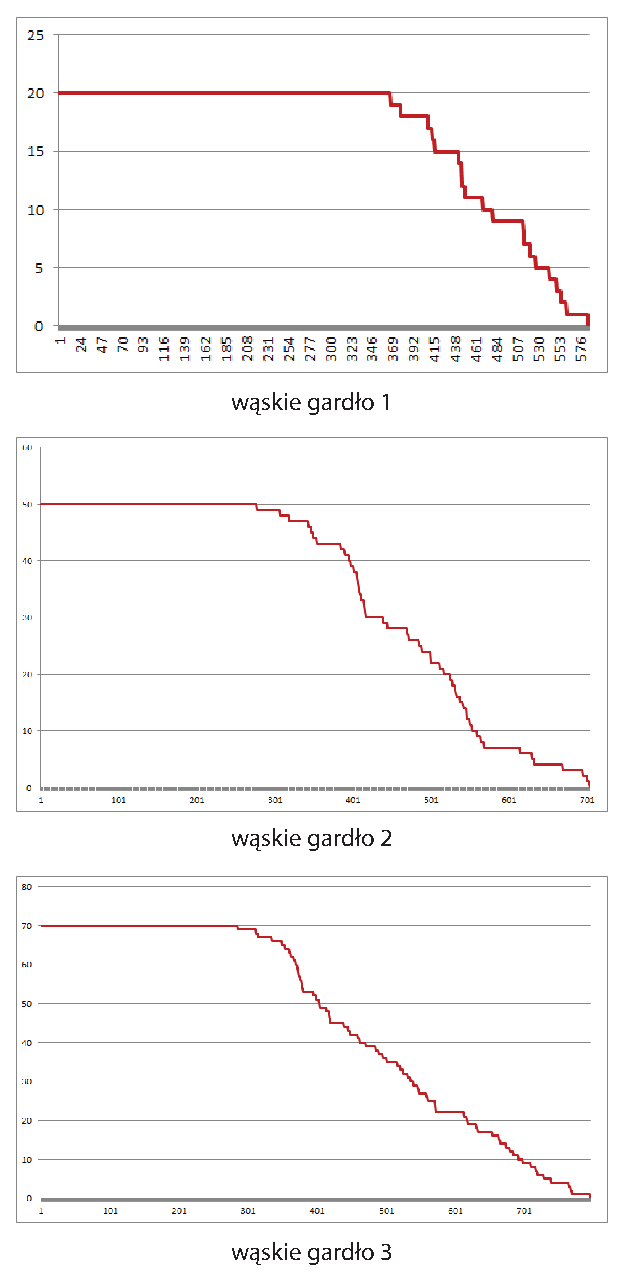
\includegraphics[width=0.4\textwidth]{iloscpieszychwaskie.eps}
\caption{Liczba pieszych w czasie - wąskie gardło}
\end{figure}
\end{samepage}

\begin{figure}
\label{figure:siatka}
\centering
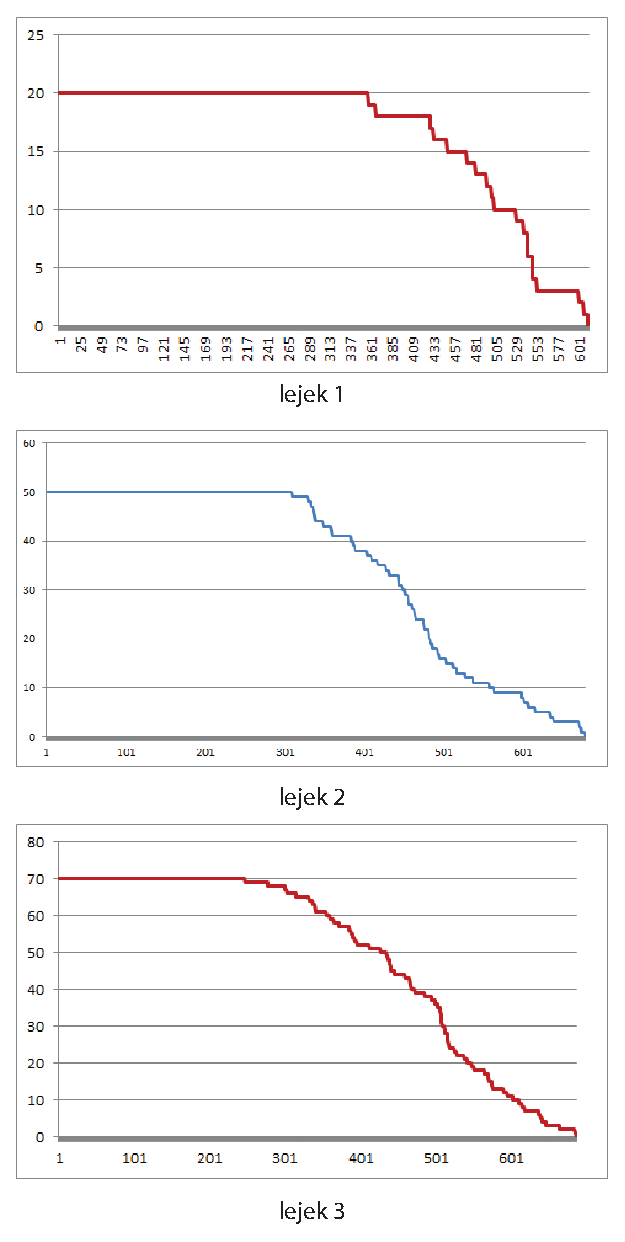
\includegraphics[width=0.5\textwidth]{iloscpieszychlejek.eps}
\caption{Liczba pieszych w czasie - lejek}
\end{figure}

\begin{figure}
\label{figure:siatka}
\centering
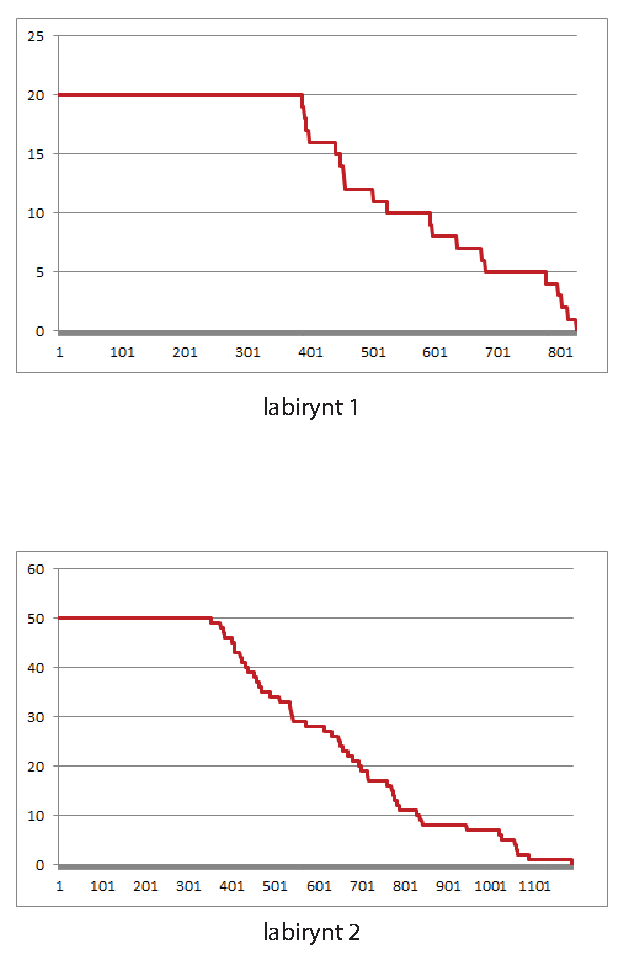
\includegraphics[width=0.5\textwidth]{iloscpieszychlabirynt.eps}
\caption{Liczba pieszych w czasie - labirynt}
\end{figure}

% \include{dodatekB}
% itd.

\printbibliography

\end{document}
